\subsection{Rezept 1 entschlüsseln}
\label{RezeptEinsEntschluesseln}

\begin{figure}
\begin{lstlisting}

\end{lstlisting}
\caption{Der verschlüsselte Text von Rezept 1}
\end{figure}

Um einen chiffrierten Text zu entschlüsseln beginnt man grundlegend mit der Kryptoanalyse. 

\subsubsection{Kryptoanalyse}

Die Kryptoanalyse hat das Ziel, Informationen über den Inhalt eines chiffrierten
Textes auch ohne Kenntnis des Schlüssels zu erhalten. Es werden verschiedene
Angriffsszenarien auf ein Kryptosystem unterschieden. Da lediglich der
chiffrierte Text bekannt war, wurde Ciphertext-Only gewählt. Es wurde mit der
Häufigkeitsanalyse begonnen.

\paragraph{Häufigkeitsanalyse}

\begin{figure}
 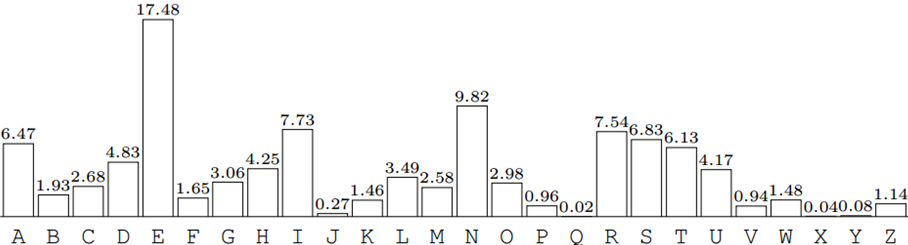
\includegraphics[width=\textwidth,keepaspectratio=true]{Images/buchstabenhaeufigkeiten_de}
 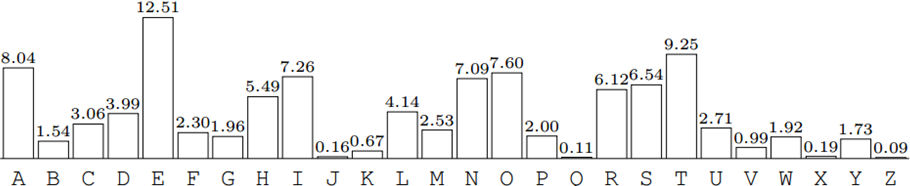
\includegraphics[width=\textwidth,keepaspectratio=true]{Images/buchstabenhaeufigkeiten_en}
 \caption{Häufigkeitsverteilung von Buchstaben im Deutschen (oben) und Englischen (unten) \cite[kap2.pdf, s. 30]{Koebler}}
 \label{fig:buchstabenhaeufigkeiten}
\end{figure}

In jeder Sprache kommen die einzelnen Buchstaben in einem ausreichend langen,
natürlichen Text in einer für die Sprache charakteristischen Häufigkeit vor
(siehe \cref{fig:buchstabenhaeufigkeiten}). Im Deutschen ist der am
häufigsten vorkommende Buchstabe das E mit einer Häufigkeit von etwa 17\%,
gefolgt vom N mit etwa 10\%.

\begin{table}[h]\footnotesize
\begin{tabular}{*{22}{r}}
  `` ``  &  `` ``  &  `` ``  &  ,  &  -  &  .  &  0  &  1  &  2  &  3  &  4  &  5  &  6  &  :  &  B  &  F  &  G  &  H & I & J  &  M \\
  10  &   10  &  126  &   13  &  1  &  8  &   10  &  4  &  3  &  2  &  3  &  3  &  1  &  1  &  1  &  5  &  2  &  1 & 1 & 2 & 4 \\
\end{tabular}

\begin{tabular}{*{22}{r}}
N  &  O  &  Q  &  R  &  T  &  U  &  X  &  Y  &  Z  &  a  &  b  &  c  &  d  &  e  &  f  &  g  &  h  &  i  &  j & m \\
3  &      5  &      3  &      4  &      1  &      2  &      1  &      1  &     10  &     58  &     10  &      1  &      1  &     38  &     25  &     44  &     33  &      4  &      8  &      5 \\
\end{tabular}

\begin{tabular}{*{20}{r}}
n  &  o  &  p  &  q  &  r  &  s  &  t  &  u  &  v  &  x  &  y  &  z  &  ˆ  &  \%  &  ¸  &  Å  \\
32  &      5  &     21  &     21  &    105  &     13  &     19  &     20  &     36  &      8  &     38  &     18  &      3  &      1  &      5  &      5  \\
\end{tabular}
\label{tab:rezept1haeufigkeit}
\end{table}

Die Häufigkeit der einzelnen Zeichen im verschlüsselten Rezept wurde mit einem
Onlinetool\footnote{\url{http://www.woerter-zaehlen.de/index.php}} gezählt und
ist in Tabelle \ref{tab:rezept1haeufigkeit} wiedergegeben.

Die Häufigkeitsanalyse ergab, dass ``e'' am häufigsten auftritt.
Es wurde als nächstes versucht, mittels der Caesar Chiffre das Wort
``Znaqryfghgra'' zu analysieren.

\paragraph{Cesar Chiffre}

Der Name Caesar-Chiffre stammt von dem gleichnamigen Feldherren Gaius Julius
Cesar (100 v. Chr. – 44 v. Chr.).1 Caesar benutzte diese sehr einfache Form der
Verschlüsselung, um militärische Nachrichten zu chiffrieren.  Es kann ein
beliebiges Alphabet verwendet werden. Die klassische Version benutzt die
Großbuchstaben A-Z. Das Alphabet wird zweimal, untereinander aufgeschrieben.
Nun wird das untere Alphabet um eine beliebige Anzahl Stellen verschoben. Diese
Anzahl von Stellen ist der Schlüsselwert der Chiffre. Eine Verschiebung um 3
nach links, also mit dem Schlüssel 3, ergibt folgende Ansicht:

\begin{lstlisting}
ABCDEFGHIJKLMNOPQRSTUVWXYZ
DEFGHIJKLMNOPQRSTUVWXYZABC

ZNAQRYFGHGRA  -> WKXNOVCDEDOX
\end{lstlisting}

\paragraph{Rot-13}

Als nächstes wurde mittels Rot-13 das Wort „ZNAQRYFGHGRA“ analysiert.

Werden als Alphabet die Buchstaben A-Z gewählt und ein Schlüssel von 13, so wird
diese Chiffre auch als Rot-13 bezeichnet. Eine Verschiebung um 13 nach links,
also mit dem Schlüssel 13, ergibt folgende Ansicht:

\begin{lstlisting}
A B C D E F G H I J K L M
N O P Q R S T U V W X Y Z

ZNAQRYFGHGRA -> MANDELSTUTEN
\end{lstlisting}

\begin{lstlisting}[caption=Quellcode rot13.c]
/*
 * Rot-13 encoder/decoder in C
 **/

#include <stdio.h>
#include <ctype.h>

int rot13( int c );

int main() {
  int c;
  while ( ( c = getchar() ) != EOF ) {
    putchar( rot13( c ) );
  }

  return 0;
}

int rot13( int c ) {
  return ( isalpha(c) )
         ? (( tolower(c) > 'm' )
           ? ( c - 13 )
           : ( c + 13 ))
         : c;
}
\end{lstlisting}

\begin{figure}
Mandelstuten
Mehl, Zucker, 2 Eier, Bittermandelaroma, gehackte Mandeln und Butter in eine große Schüssel geben.
Die Hefe in der lauwarmen Milch vollständig auflösen und ebenfalls in die Schüssel zu den anderen Zutaten schütten. Alles gut verkneten und zu einer Kugel formen.
An einem warmen Ort zugedeckt 1-2 Stunden gehen lassen, bis sich das Volumen deutlich vergrößert hat.
Den Teig nochmals gut kneten und in eine gut gefettete große Brot Form füllen.
Die zwei restlichen Eier mit etwas lauwarmer Milch verquirlen und auf den Stuten streichen.
Auf mittlerer Schiene bei 200 Grad Umluft ca. 35 Minuten backen.

Zutaten: 1000g Weizenmehl, 400ml lauwarme Milch, 60g Zucker, 1 Würfel Hefe, 4 Eier, 50g weiche Butter, 3 Tropfen Bittermandelöl,
150g gehackte Mandeln, 4 EL lauwarme Milch
\end{figure}

